%%%%%%%%%%%%%%%%%%%% author.tex %%%%%%%%%%%%%%%%%%%%%%%%%%%%%%%%%%%
%
% sample root file for your "contribution" to a contributed volume
%
% Use this file as a template for your own input.
%
%%%%%%%%%%%%%%%% Springer %%%%%%%%%%%%%%%%%%%%%%%%%%%%%%%%%%


% RECOMMENDED %%%%%%%%%%%%%%%%%%%%%%%%%%%%%%%%%%%%%%%%%%%%%%%%%%%
\documentclass[graybox]{svmult}

% choose options for [] as required from the list
% in the Reference Guide
\usepackage{amsmath}
\usepackage{booktabs}
\usepackage{mathptmx}       % selects Times Roman as basic font
\usepackage{helvet}         % selects Helvetica as sans-serif font
\usepackage{courier}        % selects Courier as typewriter font
\usepackage{type1cm}        % activate if the above 3 fonts are
                            % not available on your system
%
\usepackage{makeidx}         % allows index generation
\usepackage{graphicx}        % standard LaTeX graphics tool
                             % when including figure files
\usepackage{multicol}        % used for the two-column index
\usepackage[bottom]{footmisc}% places footnotes at page bottom

\usepackage[numbers]{natbib}
\usepackage[]{algorithm2e}

\usepackage{subfigure}
\newcommand{\stnote}[1]{\textcolor{blue}{\textbf{ST: #1}}}
\newcommand{\jgonote}[1]{\textcolor{green}{\textbf{JGO: #1}}}


% see the list of further useful packages
% in the Reference Guide

\makeindex             % used for the subject index
                       % please use the style svind.ist with
                       % your makeindex program

%%%%%%%%%%%%%%%%%%%%%%%%%%%%%%%%%%%%%%%%%%%%%%%%%%%%%%%%%%%%%%%%%%%%%%%%%%%%%%%%%%%%%%%%%

\begin{document}

\title*{Autonomously Acquiring Instance-Based Object Models}
% Use \titlerunning{Short Title} for an abbreviated version of
% your contribution title if the original one is too long
\author{John Oberlin and Stefanie Tellex}
% Use \authorrunning{Short Title} for an abbreviated version of
% your contribution title if the original one is too long
\institute{Brown University}
%
% Use the package "url.sty" to avoid
% problems with special characters
% used in your e-mail or web address
%
\maketitle

\abstract{A key aim of current research is to create robots that can
  reliably manipulate objects.  However, in many applications,
  general-purpose object detection or manipulation is not required:
  the robot would be useful if it could recognize, localize, and
  manipulate the relatively small set of specific objects most
  important in that application, but do so with very high reliability.
  Instance-based approaches can achieve this high reliability but to
  work well, they require large amounts of data about the objects that
  are being manipulated.  The contribution of this paper is a system
  that automates this data collection and adaptation process.  When
  the robot encounters a novel object, it automatically collects
  instance based models for detecting, estimating pose, and grasping
  that object.  This approach achieves the generality of
  category-based methods with the reliability of instance-based
  methods, at the cost of time spent collecting data for the model. We
  demonstrate that our approach enables an unmodified Baxter robot to
  autonomously acquire models for a wide variety of objects and then
  robustly respond to pick-and-place requests for those objects.  }


\section{Introduction}

Robotics will assist us at childcare, help us cook, and provide
service to doctors, nurses, and patients in hospitals. Many of these
tasks require a robot to robustly perceive and manipulate objects in
its environment, yet robust object manipulation remains a challenging
problem.  Systems for general-purpose manipulation are computationally
expensive and do not enjoy high accuracy on novel
objects~\citep{saxena08}.  Instance-based approaches that focus on
specific instances of objects can have higher accuracy but require
training by a human operator, which is time consuming and can be
difficult for a non-expert to perform~\citep{ork14, lai11, lai11a}.
Existing approaches to autonomously learn 3D object models still
require expensive ICP-based methods to localize objects, which are
susceptible to local minima and take time to
converge~\citep{krainin11}.

To address these problems, we present an approach that captures the
high accuracy of instance-based methods without the need for manually
acquiring training data by enabling a robot to learn to identify and
grasp on a per object basis. Our grasping and perception pipeline uses
standard computer vision techniques to perform data collection,
feature extraction, and training, along with active visual servoing
for localization.  Using our algorithm, the robot detects candidate
objects for training using a depth sensor, then actively collects
view-based visual templates to perform robust instance-based object
detection, pose estimation and grasping models using visual servoing.
Because our camera can move with seven degrees of freedom, the robot
can collect large quantities of data leading to simple visual models
that perform with high accuracy.  Our approach is enabled by three
components: our end-to-end algorithm for collecting view-based
training data with supervision obtained from a higher-reliability
depth sensor, which is supported by a simple and robust method for
determining candidate grasps using a depth sensor mounted on a
seven-degree-of-freedom arm, along with an approach for autonomously
and reliably finding object bounding boxes once the object is on a
background such as a floor or table.

\section{Overview and Approach}
Robots can interact with the physical world and collect multiple images
for processing. We exploit this fact to make some computer vision tasks
easier by physically adding invariance rather than hand engineering
features.

Our approach lets us use rich but inconvenient depth sensors once at learning
time and then exploit the knowledge they provide by using only an RGB
camera at run time.

\subsection{Invariance in Images}
A theme in computer vision and pattern recognition Is the notion of invariance.
We like to detect objects anywhere in an image, invariant to their positions.
We want to find the spoon no matter which direction it is pointing, invariant
to its pose. Shadows and reflections can be confusing so we want to be
invariant to lighting. What if you could add invariance to an image? With a
robot you can.

\begin{table}
\begin{tabular}{ccc}
\toprule
Subsystem      &  Invariance(s) Addressed\\
\midrule
Canny Servo    &  Position\\
Gradient Servo &  Orientation\\
Light Map      &  Lighting Gain, Bias, Reflection, Shadow\\
\bottomrule
\end{tabular}
\end{table}

Canny Autotune is robotic because we have access to the environment and can
take additional images.

We can actively light the area with white or IR light (Kinect, for instance) to
get some invariance to lighting. The IR rangefinder we use is active.

SIFT features give some invariance to scale, as their name implies. BoW models
give invariance to small model deformation. For invariance to large
deformations, significant and expensive modeling such as DPM or CNN is
required. 

We can use our freedom as roboticists (all 7 degrees of it) to add invariance
to a task not by addressing the features or models as much prior work does, but
by adding it to the data at training and inference. 

Collecting the data in a timely fashion both requires and facilitates a
relatively tight loop of control over the robot’s joint states. Canny servoing
will have an auto-threshold feature that adds lighting invariances to a fast
saliency map. The resulting movement yields invariance to large translations.
Gradient servoing provides invariance to orientation and small translations.

Light Map is what averaging before the gradient servo will become. We map the
projection of the object onto the table in physical coordinates, aggressively
ignoring reflections and shadows, moving to get a better view and fill in gaps.
Then we use that map for inference, our immediate cases being that we treat it
as an image and classify it then feed it into gradient servo. 

Deterministic light mapping is a nice non-parametric method, but you could
imagine an online method that iteratively estimates the orientation of the
object, uses prior knowledge of the appearance combined with accumulated
measurements to construct the light map, then uses that map to estimate the
orientation of the object, and repeats until convergence. Such a method might
be called Light SLAM.

\subsection{Sensors}
By developing systems that work well in real time in simple environments with
specific objects, we obtain the capacity to collect enough labeled data to
train systems with the ability to generalize and perform well in more
complicated, cluttered environments. This approach also lets us get a head
start with the logistical problems involved in transforming theory to practice.

Infrared (IR) imaging can be useful for segmenting and determining geometry and
many devices (including the range finder we employ) are active in that they
shine IR light and measure the return signal. The rangefinder’s readings are
somewhat invariant to color and material while motionless, but show anisotropic
artifacts near edges and during movement. None the less, for the most part the
readings are good enough for us to infer grasps. 

Transparent materials are invisible, reflective materials induce artifacts, and
dark materials are worse during movement. To overcome these issues on other
devices, people have spraypainted objects to make them permanently well
behaved. This works to a degree but really breaks the suspension of disbelief
and is inappropriate for domestic application. We developed a temporary
contrast agent that can be applied safely and easily removed. We scan objects
in IR once during training and use that scan during inference so that we can
pick things up using only RGB data and do not require a permanent agent.

We use a two phase contrast agent consisting of a binding phase and a
conditioning phase. The conditioning phase scatters and reflects incoming IR
light and the binding phase attach the conditioner to the surface of the
object. For binders we investigated vaseline, zinc oxide ointment (diaper
creme), and Aquanet hairspray. The only conditioner we tried was wheat flour,
but you could substitute cornstarch or baking powder in a pinch. We settled on
the Aquanet because it was fast, not too messy, and as the shell of flour
hardened it eventually shrank so much that it detached cleanly on its own from
many surfaces after 60 minutes. Aquanet may be inappropriate for some surfaces,
in which case water could serve as a binder. In extreme situations, since the
scan is top down and only needs to detect normal (horizontal) surfaces, you can
run a scan with no binding phase since a dusting of powder will settle on
desirable surfaces. This could even be seen as physical feature detection.

\subsection{Purpose}
\jgonote{I know some of this doesn't really belong but I had these thoughts
and wanted to add them in case they are useful for, say, future work.}
One purpose of this system is to investigate an approach to gathering data and
training models that enable multiple robotic platforms to robustly detect and
manipulate novel objects and to improve in ability over time. The approach
consists of three phases.

In the first phase, the system trains only instance level models of objects and
collects data on those objects as it manipulates them, using heuristic
proposals for grasp points and confidence bounds for learning. In the second
phase, the system uses the data collected from instance level models to train
category level detectors for object class and grasp locations. During the
second phase, the system still uses its parent proposals during operation but
it continuously evaluates the performance of the juvenile category level
detectors. When the category level detectors are comparable to the parent
detectors, the third phase begins and the system uses its trained category
models instead of the originally provided parent heuristics. 

In addition to being a convenient way to initially train models, this three
fold process is a general method for bootstrapping a new classifier to replace
an old one without taking the system offline.





\section{Grasping System}

\begin{figure}
\subfigure[RGB Image of an object.]{
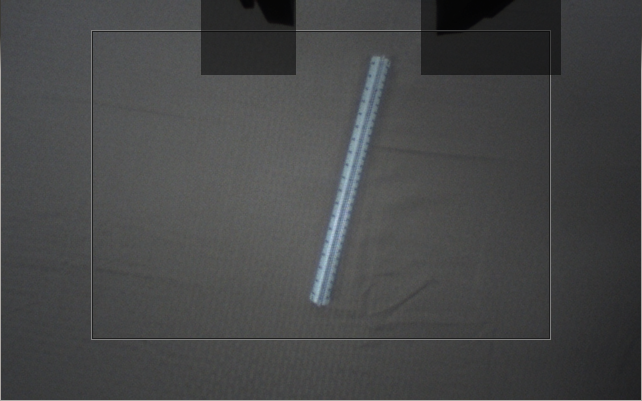
\includegraphics[width=0.24\linewidth]{figures/ruler_01_initial.png}
}%
\subfigure[Bounding box extracted for the object.]{
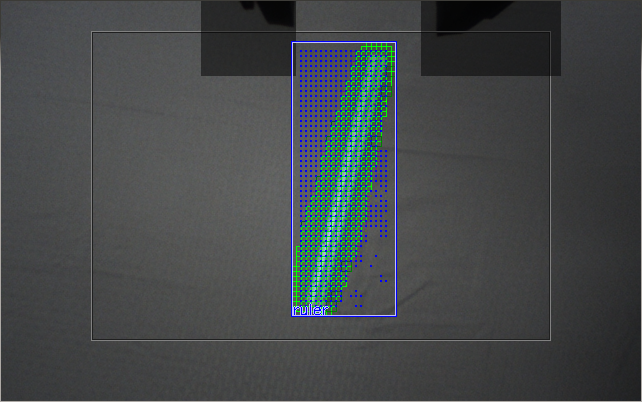
\includegraphics[width=0.24\linewidth]{figures/ruler_02_labeled.png}
}%
\subfigure[Gradient image of the object.]{
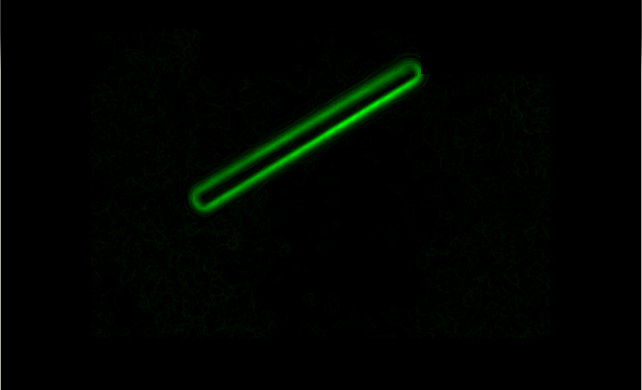
\includegraphics[width=0.24\linewidth]{figures/ruler_04_gradient.png}
}%
\subfigure[Stored gradient image overlayed on the object image after servoing.]{
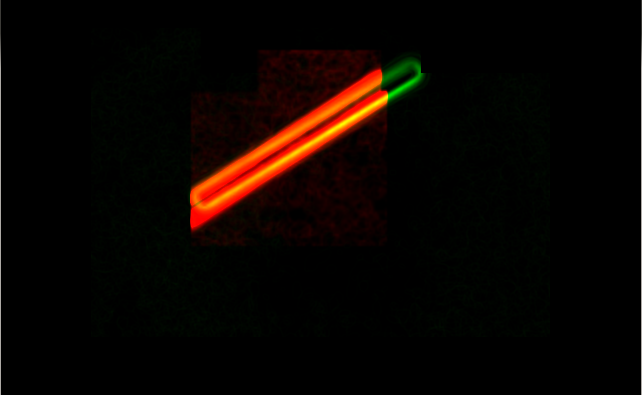
\includegraphics[width=0.24\linewidth]{figures/ruler_05_gradient_overlay.png}
}%

\caption{Results at each phase of the localization pipeline.\label{fig:images}}
\end{figure}

We first describe our instance-based object detection and pose
estimation pipeline, which uses standard computer vision algorithms
combined to achieve a simple software architecture, a high frame rate,
and high accuracy at recognition and pose
estimation.  Section~\ref{sec:training} describes our
approach to enabling a robot to autonomously collect the data needed
to perform grasping with this pipeline.

Our recognition pipeline takes video from the robot, proposes a small
number of candidate object bounding boxes in each frame, and
classifies each candidate bounding box as belonging to a previously
encountered object class. Our object classes consist of object
instances rather than pure object categories.  Using instance
recognition means we cannot reliably detect categories, such as
``mugs,'' but the system will be able to detect, localize, and grasp
the specific instances for which it has models with much higher speed
and accuracy.  A visualization of data flow in the pipeline appears in
Figure~\ref{fig:system} while Figure~\ref{fig:images} shows results
from each phase of the localization pipeline.  For each module, we
formalize its input, output, and reward function; each component can
have multiple implementations which better for different objects.  The
following sections describe how we can use this pipeline to learn
which implementation to use for specific objects; this learning
dramatically speeds up performance.

\begin{figure}
\centering
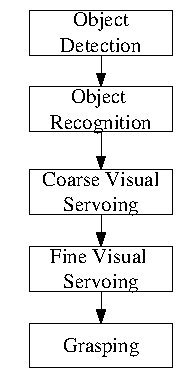
\includegraphics{figures/system.pdf}
\caption{Data flow in our grasping system.\label{fig:system}\stnote{maybe combine with figure 1}}
\end{figure}

\subsection{Object Detection}
\label{sec:detection}

The goal of the object detection component is to extract bounding
boxes for objects in the environment from a relatively uniform
background.  The robot uses object detection to identify regions of
interest for further processing.  The input of the object detection
component is an image, $I$; the output is a set of candidate bounding
boxes, $B$.  

Our object detection approach uses a modified Canny algorithm which
terminates before the usual non-maximal suppression
step~\citep{canny86}.  We start by converting $I$ to YCbCr opponent
color representation.  Then we apply $5 \times 5$ Sobel derivative
filters~\citep{sobel95} to each of the three channels and keep the
square gradient magnitude. We take a convex combination of the three
channels, where Cb and Cr and weighted the same and more heavily than
Y because Y contains more information about shadows and specular
information which adds noise.  After this we downsample, apply the two
Canny thresholds, and find connected components.  If a connected
component is contained in another, we discared the contained
component.  We throw out boxes which do not contain enough visual data
to classify.  We generate a candidate bounding box for each remaining
component by taking the smallest box which contains the component.

\subsection{Object Classification}
\label{sec:recognition}

The object recognition module takes as input a bounding box, $B$, and
outputs a label for that object, $c$, based on the robot's memory.
This label is used to identify the object and look up other
information about the object for grasping further down the pipeline.

For each object $c$ we wish to classify, we gather a set of example
crops $E_c$ which are candidate bounding boxes (derived as above)
which contain $c$. We extract dense SIFT features ~\citep{lowe99} from
all boxes of all classes and use k-means to extract a visual
vocabulary of SIFT features ~\citep{szeliski10}. We then construct a
Bag of Words feature vector for each image and augment it with a histogram of
colors which appear in that image.  The augmented feature vector is
incorporated into a k-nearest-neighbors model which we use to classify
objects at inference~\citep{szeliski10}. We use kNN because our
automated training process allows us to acquire as much high-quality
data as necessary to make the model work well, and kNN supports direct
matching to this large dataset.  

\subsection{Pose Estimation}

We use the image gradient for object detection and pose
estimation. During object detection, the gradient of the whole image
is the first step in the Canny pipeline.  For pose estimation, we
require a crop of image gradient of the object at a specific, known
pose.

We denote the gradient by
\begin{align}
\Delta I = \left( \frac{\partial I}{\partial x}, \frac{\partial I}{\partial y} \right)
\end{align}

As in bounding box proposal, we approximate the gradient using $5
\times 5$ Sobel derivative filters~\citep{sobel95}, but we use a
different convex combination of the channels which focuses even less
on the Y channel.  Camera noise in the color channels is
significant. To cope with the noise, we marginalize the gradient
estimate over several frames taken from the same location, providing a
much cleaner signal which matches more robustly.  To estimate pose, we
rotate our training image and find the closest match to the image
currently recorded from the camera, as detected and localized via the
pipeline in Section~\ref{sec:detection} and~\ref{sec:recognition}.

In order to match our template image with the crop observed at pick time,
we remove the mean from and $L^2$ normalize the template and the crop.
Removing the mean provides invariance to bias, and normalizing introduces
invariance to scaling, which both help account somewhat
for lighting. 

\subsection{Identifying Grasp Points}

To identify a grasp points, we combine a depth map of the object with
a model of the gripper.  The depth map appears in
Figure~\ref{fig:depth_map} and is acquired by moving the rangefinder
on the arm through a raster scan over the object.  The grasp model
scores each potential grasp according to a linear model of the gripper
to estimate grasp success. A default algorithm picks the
highest-scoring grasp point using hand designed linear filters, but
frequently this point is not actually a good grasp, because the object
might slip out of the robot's gripper or part of the object may not be
visible in IR.  The input to this module is the 3d pose of the object,
and the output is a grasp point $(x, y, \theta)$; at this point we
assume only crane grasps rather than full 3d grasping, where $\theta$
is the angle which the gripper assumes for the grasp.



\subsection{Closed-Loop Grasping}

To grasp an object, we first scan the work area by moving the camera
until the object is detected and recognized.  Then we perform active
visual servoing to move the arm directly above the object.  Next, we
perform orientation servoing using the pose estimation
algorithm. Because these components are instance-based, they report
position and orientation with high accuracy, enabling us to use a
proportional controller (with no derivative or integral terms) to move
the arm into position.  Last, we move the arm to the desired grasp
location, close the gripper, and pick up the object.


\subsection{Autonomous Training}
\label{sec:training}

An object model in our framework consists of the following elements,
which the robot autonomously acquires:
\begin{itemize}
\item cropped object templates (roughly 200), $t^1 ... t^K$
\item depth map, $D$, which consists of a point cloud, $(x, y, z, r, g, b)^{i,j}$.
\item cropped gradient templates at different heights, $t_0 ...  t^M$
\end{itemize}

The robot collects gradient images by servoing to the center of the
extracted bounding box for the object, described in
Section~\ref{sec:detection}, and then recording a gradient image at
several different heights.  It records each image for several frames
to average away noise from the camera.  Gradient images for the ruler
appear in Figure~\ref{fig:gradient}.  

Next it acquires a depth image.  Normally this image could be acquired
from an RGB-D sensor such as the Kinect.  However, in order to make
our approach run on a stock Baxter robot with no additional sensing,
we acquire a depth scan using Baxter's IR sensor, turing the arm into
a seven degree of freedom, one-pixel depth sensor.  We perform an IR
scan scan 2cm above the tallest height, but we set it manually to save
time.  Additionally we set the height of the arm for the initial servo
to acquire the object.  After acquiring visual and IR models for the
object at different poses of the arm,

Once the object has been moved to
a known pose, we acquire the object model by moving the camera around
the object, extracting bounding boxes from the resulting imgages, and
storing the resulting crops.  Figure~\ref{fig:ruler_rgb} shows RGB
images automaticaly collected for one object in our dataset.


\begin{figure}
\subfigure[Cropped RGB images.\label{fig:ruler_rgb}]{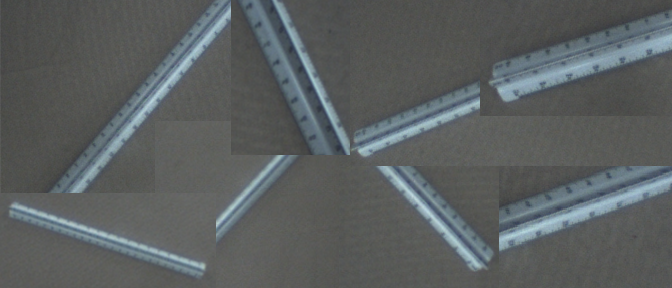
\includegraphics[width=1\linewidth]{figures/ruler_collage.png}}

\subfigure[Depth map.]{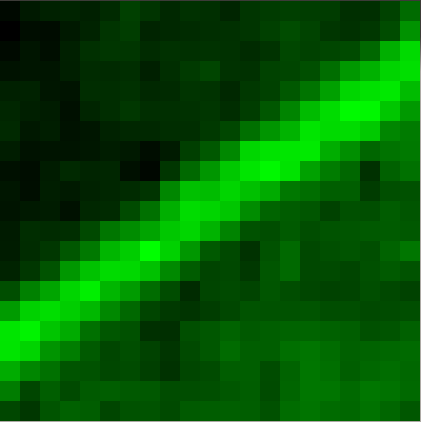
\includegraphics[width=0.4\linewidth]{figures/ruler_06_depth.png}}
\subfigure[\label{fig:gradient}Gradient map.]{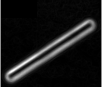
\includegraphics[width=0.4\linewidth]{figures/ruler_07a_aerialGradient.png}}

\caption{An object model in our pipeline.\label{fig:ruler_model}}
\end{figure}


\section{Evaluation}

We evaluate our approach in two ways, first at mapping a tabletop
scene, and second by assessing picking accuracy.  Video showing our
training and grasping pipeline is available at
\url{https://www.youtube.com/watch?v=xfH0B3g782Y}.


\subsection{Mapping Accuracy}

Mapping assesses the ability of our robot to accurately localize and
label objects in a tabletop scene.  We assess performance by creating
scenes containing a subset of the objects used in our evaluation.  The
robot maps the scene by maintaining a data structure for each cell in
its work space, at approximately 1cm resolution and recording the last
time that cell was observed by the camera.  It samples a new cell
uniformly from the set of oldest cells, moves to that location, then
runs the detection step.  If it sees an object, it servos to that
object, then adds the object's bounding box and category to the map.
Figure~\ref{fig:map} shows the map created in this way for a tabletop
scene.

\begin{figure}
\subfigure[Tabletop scene.]{\parbox{0.5\linewidth}{~\\~\\~\\~\\}}
\subfigure[Map created from the scene.]{\parbox{0.5\linewidth}{~\\~\\~\\~\\}}
\label{fig:map}
\end{figure}

We report precision and recall for each object in the scene.
Precision means that if the system associated that object with a
bounding box, it correctly labeled it.  Recall means that the object
associated each object in the scene with a bounding box with a correct
label.

\subsection{Picking Accuracy}

\begin{figure}
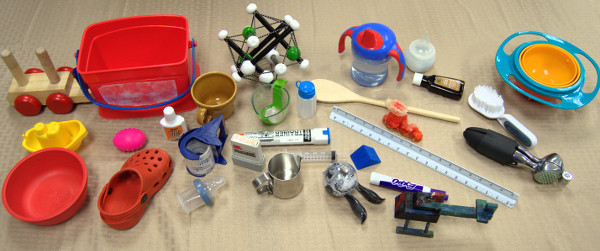
\includegraphics[width=1\linewidth]{figures/object_glory_shot.jpg}
\caption{The objects used in our evaluation.\label{fig:object_glory_shot}}
\end{figure}

We evaluated our system by training models for a diverse set of
objects and assessing picking accuracy.  The objects in our evaluation
appear in Figure~\ref{fig:object_glory_shot}.

After the robot detects an initially successful grab, it shakes the
object vigorously to ensure that it would not fall out during
transport. After releasing the object and moving away, the robot
checks to make sure the object is not stuck in its gripper. If the
object falls out during shaking or does not release properly, the
grasp is recorded as a failure. If the object is stuck, the robot
pauses and requests assistance before proceeding.

Most objects have more than one pose in which they can stand upright
on the table. If the robot knocks over an object, the model taken in
the reference pose is no longer meaningful. Thus, during training, we
monitored the object and returned it to the reference pose whenever
the robot knocked it over. In the future, we aim to incorporate
multiple components in the models which will allow the robot to cope
with objects whose pose can change during training.  We report the
performance of the robot at picking after training models for the
system.


\begin{table}
\small
\centering
\begin{tabular}{cc}
\toprule
Object		    & \# Picks/\# Tries\\
\midrule
% too easy
Brush    	    & 10/10\\
Red Bowl    	    & 10/10\\
Shoe    	    & 10/10 \\
Whiteout    	    & 10/10 \\
Yellow Boat    	    & 9/10  \\
Syringe    	    & 9/10  \\
Packing Tape        & 9/10 \\
Purple Marker       & 9/10 \\
Stamp    	    & 8/10  \\
Toy Egg    	    & 8/10  \\
Dragon    	    & 8/10  \\
Epipen    	    & 8/10  \\
Icosahedron    	    & 7/10  \\
Wooden Spoon        & 7/10  \\
Blue Salt Shaker    & 6/10  \\
\bottomrule
\end{tabular}
~~~~~~~~~~~~~~~~~~\begin{tabular}{cc}
\toprule
Object		    & \# Picks/\# Tries\\
\midrule
Metal Pitcher       & 6/10  \\
Ruler    	    & 6/10  \\
Vanilla	   	    & 5/10  \\
Red Bucket    	    & 5/10\\
Wooden Train        & 4/10  \\
Clear Pitcher       & 4/10  \\
Mug    		    & 3/10  \\
Helicopter    	    & 2/10  \\
Round Salt Shaker   & 1/10  \\
Big Syringe    	    & 1/10  \\
Bottle Top    	    & 0/10  \\
Garlic Press        & 0/10  \\
Gyro Bowl    	    & 0/10  \\
Sippy Cup    	    & 0/10  \\
Triangle Block      & 0/10  \\
\bottomrule
\end{tabular}

\caption{Results from the robotic evaluation. We tested on 30 objects.
  Overall performance is 165 picks of 300 tries, or
  55\%. \label{table:robot_results}}
\end{table}

Our evaluation demonstrates that for many objects, the system obtains
a very high grasp success rate.  Objects failed for several reasons.
Some objects, such as the garlic press, were quite heavy, at the edge
of the robot's capability to lift.  Other objects, such as those in
Figure~\ref{fig:poor_ir} are poorly visible in IR.  In our other
work~\citep{oberlin15}, we showed that we could improve the robot's
grasp rate on these objects by actively picking and learning better
grasp points.  This demonstrates the advantage of our vision-based
approach, which uses IR only at grasp proposal time, and not at
inference time; once a good grasp is obtained, high-quality grasps can
be inferred at pick time.

Besides our learning approach, we also found that applying a contrast
agent significantly improves grasp success.  For example, for the two
objects in Figure~\ref{fig:poor_ir}, performance using a contrast
agent raises to XX.

\begin{table}
\begin{tabular}{ccc}
Object		    & \# Picks/\# Tries (no contrast agent) &\# Picks/\# Tries (contrast agent)\\
Round Salt Shaker   & 1/10  & \\
Bottle Top    	    & 0/10  & \\
\midrule
Overall             &       &\\
\bottomrule
\end{tabular}
\end{table}

\begin{figure}
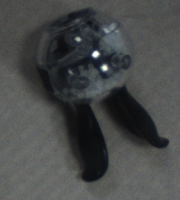
\includegraphics[width=0.3\linewidth]{figures/saltshaker.png}
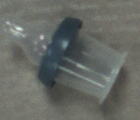
\includegraphics[width=0.3\linewidth]{figures/bottletop.png}
\caption{Poorly performing objects because they are not well visible
  in IR.\label{fig:poor_ir}}
\end{figure}

\section{Related Work}

\label{sec:relatedwork}
\jgonote{I can do a little survey here on standard approaches for adding
invariance in computer vision and attempt to find some approaches in robotics
that add invariance in atypical ways.}

\citet{bohg13} survey data-driven approaches to grasping.  Our
approach can be thought of as a pipeline for automatically building an
experience database consisting of object models and known good grasps,
using analytic approaches to grasping unknown objects to generate a
grasp hypothesis space and using our bandit-based method for trying
grasps and learning instance-based distributions for the grasp
experience database.  In this way our system achieves the best of both
approaches: models for grasping unknown objects can be applied; when
they do fail, the system can attempt to recover by trying grasps and
adapting itself based on that specific object.  

\citet{ude12} described an approach for detecting and manipulating
objects to learn models.  It uses a bag of words model and learns to
detect the objects.  It does not learn a model for grasping.
\citet{schiebener13} describes an extension that also does model
learning.  The robot pushes the object and then trains an object
recognition system.  It does not use a camera that moves and does not
grasp.
\citet{schiebener12} discovers and grasps unknown objects.

Summary: 
\begin{itemize}
\item People doing SLAM.  \citet{wang07, gallagher09}, 
\item People doing 3d reconstruction.   \citet{krainin11, banta00}
\item People doing big databases for category recognition.  \citet{kent14a, kent14, lai11a, goldfeder09}
\item Object tracking in vision (typically surveillance).
\item POMDPs for grasping.  \citet{platt11, hsiao10}
\item People doing systems.  \citet{hudson12, ciocarlie14}
\end{itemize}




Crowd-sourced and web robotics have created large databases of objects
and grasps using human supervision on the web~\citep{kent14a, kent14}.
These approaches outperform automatically inferred grasps but still
require humans in the loop.  Our approach enables a robot to acquire a
model fully autonomously, once the object has been placed on the
table.

\citet{zhu14} created a system for detecting objects and estimating
pose from single images of cluttered objects.  They use KinectFusion
to construct 3d object models from depth measurements with a
turn-table rather than automatically acquiring models.

\citet{chang12} created a system for picking out objects from a pile
for sorting and arranging but did not learn object models.  

next-best view planning~\citep{kriegel11}

\citet{nguyen14} learn to manipulate objects such as a light switch or
drawer with a similar self-training approach.  Our work learns visual
models for objects for autonomous pick-and-place rather than to
manipulate objects.

Developmental/cognitive robotics~\citep{lyubova13, kraft10r}

\citet{banta00} constructs a prototype 3d model from a minimum number
of range images of the object.  It terminates reconstruction when it
reaches a minimum threshold of accuracy.  It uses methods based on the
occluded regions of the reconstructed surface to decide where to place
the camera and evaluates based on the reconstruction rather than pick
up success.  \citet{krainin11} present an approach for autonomous
object modeling using a depth camera observing the robot's hand as it
moves the object.  This system provides a 3d construction of the
object autonomously.  Our approach uses vision-based features and
evaluates based on grasp success.  Eye-in-hand laser
sensor.~\citep{aeotti14}

\stnote{Need to find the instance-based work that Erik mentioned when
  he said it was a ``solved problem.''}

\citet{velez11} created a mobile robot that explores the environment
and actively plans paths to acquire views of objects such as doors.
However it uses a fixed model of the object being detected rather than
updating its model based on the data it has acquired from the
environment.

Methods for planning in information space \citep{he08, atanasov13,
  prentice09} have been applied to enable mobile robots to plan
trajectories that avoid failures due to inability to accurately
estimate positions.  Our approach is focused instead on
object detection and manipulation, actively acquiring data for use
later in localizing and picking up objects. \stnote{May need to say
  more here depending on what GRATA actually is.}


Early models for pick-and-place rely on has been studied since the
early days of robotics~\citep{brooks83, lozano89}.  These systems
relied on models of object pose and end effector pose being provided to the
algorithm, and simply planned a motion for the arm to grasp.  Modern
approaches use object recognition systems to estimate pose and object
type, then libraries of grasps either annotated or learned from
data~\citep{saxena08, goldfeder09, morales03}.  These approaches
attempt to create systems that can grasp arbitrary objects based on
learned visual features or known 3d configuration.  Collecting these
training sets is an expensive process and is not accessible to the
average user in a non-robotics setting.  If the system does not work
for the user's particular application, there is no easy way for it to
adapt or relearn.  Our approach, instead, enables the robot to
autonomously acquire more information to increase robustness at
detecting and manipulating the specific object that is important to
the user at the current moment.

Visual-servoing based methods~\citep{chaumette06} \stnote{Need a whole
  paragraph about that. }

\stnote{\citet{ciocarlie14} seems highly relevant, could not read from
  the train's wifi.}  Existing work has collected large database of
object models for pose estimation, typically curated by an
expert~\citep{lai11}.  \citet{kasper12} created a semiautomatic system
that fuses 2d and 3d data, but the setup requires a special rig
including a turntable and a pair of cameras.  Our approach requires an
active camera mounted on a robot arm, but no additional equipment, so
that a robot in the home can autonomously acquire new models.

\citet{collect14} describes an approach for lifelong robotic object
discovery, which infers object candidates from the robot's perceptual
data.  This system does not learn grasping models and does not
actively acquire more data to recognize, localize, and grasp the
object with high reliability.  It could be used as a first-pass to
our system, after which the robot uses an active method to acquire
additional data enabling it to grasp the object.  Approaches that
integrate SLAM and moving object tracking estimate pose of objects
over time but have not been extended to manipulation~\citep{wang07,
  gallagher09, salas-moreno13, selvatici08}.

Our approach is similar to the philosophy adopted by Rethink Robotic's
Baxter robot, and indeed, we use Baxter as our test
platform~\citep{fitzgerald13}.  \stnote{Haven't actually read this
  paper, just making stuff up based on Rod's talks.  Should read the
  paper and confirm.}  Baxter's manufacturing platform is designed to
be easily learned and trained by workers on the factory floor.  The
difference between this system and our approach is we rely on the
robot to autonomously collect the training information it needs to
grasp the object, rather than requiring this training information to
be provided by the user.


Robot systems for cooking~\citep{bollini12, beetz11} or furniture
assembly~\citep{knepper13} use many simplifying assumptions, including
pre-trained object locations or using VICON to solve the perceptual
system.  We envision vision or RGB-D based sensors mounted on the
robot, so that a person can train a robot to recognize and manipulate
objects wherever the robot finds itself.

Approaches to plan grasps under pose uncertainty~\citep{stulp11} or
collect information from tacticle sensors~\citep{hsiao10} using
POMDPs.  \citet{plat11} describe new algorithms for solving POMDPs by
tracking belief state with a high-fidelity particle filter, but using
a lower-fidelity representation of belief for planning, and tracking
the KL divergence.

\citet{hudson12} used active perception to create a grasping system
capable of carrying out a variety of complex tasks.  Using feedback is
critical for good performance, but the model cannot adapt itself to
new objects.

\section{Conclusion}

The contribution of this paper is a system for automatically acquiring
instance-based models of objects.  We have demonstrated our system's
performance at creating a map of objects in its local environment as
well as by assessing the pick accuracy of objects on a challenging
test set.  Our approach runs on a stock Baxter robot and does not
require any additional sensing, and we plan to release the source code
once the paper is accepted, enabling anyone with a Baxter to train
models using our approach.

We plan to extend our framework so that object models are
automatically uploaded to a common database.  As more and more models
are collected, containing RGB image crops, point clouds, and logs of
grasp success rates at different geometries, this data set will
provide a unique opportunity to train new category-based models for
general detection and grasping, training on data of multiple views of
many instances of individual objects.

A signficiant limitation of our existing system is the requirement for
an object to always be in a consistent position with respect to the
table.  In our pick-and-place evaluation, we reset the object if it
fell down (for example, if a salt shake fell on its side).  Our next
goal is to automatically detect these object modes and acquire
detection, localization, and grasping models for them as well using
active exploration.  Next, the robot can learn to transition an object
from one mode to another, so that it can learn to robustly manipulate
the objects.  Using this framework, the system will be capable of
autonomously learning grasping models over a long period of time,
significantly increasing the size of the dataset collected and thus
robustness.

\bibliographystyle{plainnat}
\bibliography{main}

\end{document}
